\clearpage

\lehead[]{\sf\hspace*{-2.00cm}\textcolor{white}{\colorbox{lightblue}{\makebox[1.60cm][r]{\thechapter}}}\hspace{0.17cm}\textcolor{lightblue}{\chaptertitle}}
\rohead[]{\textcolor{lightblue}{\chaptertitle}\sf\hspace*{0.17cm}\textcolor{white}{\colorbox{lightblue}{\makebox[1.60cm][l]{\thechapter}}}\hspace{-2.00cm}}
%\chead[]{}
\rehead[]{\textcolor{lightblue}{AvHG, Inf, My}}
\lohead[]{\textcolor{lightblue}{AvHG, Inf, My}}

\lstset{style=myJava}

\section{Komplexere Dialogelemente}

\subsection{Allgemein}

Swing unterscheidet zwischen den Daten und ihrer Darstellung. Für die
Swing-Komponenten gibt es jeweils ein Datenmodell (Model). Das ist uns bisher
bei den einfachen Komponenten, wie \myClass{JLabel} und \myClass{JTextField}
noch nicht begegnet\footnote{Das stimmt nicht ganz: Im Abschnitt zur
Ereignisbehandlung für die Klasse \myClass{JTextField} wurde bereits einmal
dessen Datenmodell erwähnt/benutzt.}.
Aber jetzt ...

\subsection{\myClass{JList}}

Die Klasse \myClass{JList} ermöglicht es eine Liste von Daten in einem
Dialogelement anzuzeigen. Das kann im einfachsten Fall eine Liste von
\myClass{Strings} sein. Es könnten aber auch komplexere Datensätze -- etwa eine
Kombination von Bildern und Text -- sein.

\begin{minipage}{0.35\textwidth}
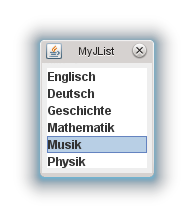
\includegraphics[width=1.0\textwidth]{./inf/SEKII/24_Java_GUI-Komponenten/JList.png}
\end{minipage}
\begin{minipage}{0.65\textwidth}
Im einfachsten Fall, nämlich der Präsentation von statischen (unveränderlichen)
Listen kommt man noch ohne Model aus. Man muss bei der Erzeugung der
\myClass{JList}-Komponente nur festlegen, welcher Datentyp abgebildet werden
soll. Etwa so:

\begin{lstlisting}
String[] faecher = {"Englisch", "Deutsch", "Geschichte", 
                    "Mathematik", "Musik", "Physik"};
JList<String> listFaecher = new JList<String>(faecher);
\end{lstlisting}

In Spitzen Klammern wird dabei der Datentyp angegeben (ab JDK7).

Mit der Methode \lstinline|getSelectedValue()| aus der Klasse \myClass{JList}
bekommt man das vom Benutzer ausgewählte Element der Liste zurück:

\begin{lstlisting}
String gewaehltesFach = listFaecher.getSelectedValue();
\end{lstlisting}
\end{minipage}


\subsubsection{\myClass{ListSelectionModel}}

Der Benutzer kann mit der Maus Einträge aus der Liste auswählen. Dabei kann
festgelegt werden, ob er nur einzelne oder auch mehrere Einträge gleichzeitig
auswählen kann:

\begin{lstlisting}
listFaecher.setSelectionMode(ListSelectionModel.SINGLE_SELECTION);
\end{lstlisting}

legt fest dass nur jeweils ein Listen-Eintrag ausgewählt werden kann. Alternativ
kann man auch

\lstinline|SINGLE_INTERVAL_SELECTION| und
\lstinline|MULTIPLE_INTERVALL_SELECTION|

angeben. Damit kann der Benutzer später einzelne oder eben auch mehrere
zusammenhängende Bereiche aus der Liste auswählen.

\subsubsection{DefaultListModel}

Oft ist es jedoch nötig, die Daten in der Liste zu verändern (etwa Daten
hinzufügen oder löschen). Diese Flexibilität wird über die Klasse
\myClass{DefaultListModel} erreicht: Im Model wird festgelegt um was für Daten
es sich handelt. Das Model ist auch dafür zuständig mit diesen Daten zu
arbeiten. Ohne Datenmodell auch keine dynamischen (veränderliche) Listen! Die
Definition des Datenmodells ist also oft der erste Schritt um mit einer
\myClass{JList}-Komponente arbeiten zu können.

\begin{lstlisting}
String[] faecher = {"Englisch", "Deutsch", "Geschichte", 
                    "Mathematik", "Musik", "Physik"};
DefaultListModel<String> faecherliste = new DefaultListModel<String>();
JList<String> listFaecher = new JList<String>(faecherliste);
\end{lstlisting}

Wenn man die \myClass{JList}-Komponente nun darstellen lassen würde, wäre sie
allerdings noch leer! Dank des Models ist unsere Liste ja nun dynamisch. Als
erstes werden wir sie also mit den alten Daten befüllen:

\begin{lstlisting}
for (String fach: faecher) {
    faecherliste.addElement(fach);
}
\end{lstlisting}

Die Methode \lstinline|addElement()| aus der Klasse \myClass{DefaultListModel}
erledigt dabei nicht nur das Einfügen der einzelnen Fächer in unsere Liste (es
hängt das neue Element einfach an die bestehende Liste an), sondern sorgt
gleichzeitig (und automatisch) dafür, dass alle Komponenten, die dieses Model
benutzen die aktualisierte Liste darstellen.

Weitere wichtige Methoden aus der Klasse \myClass{DefaultListModel} sind:

\bgroup
\def\arraystretch{1.2}
\begin{tabularx}{\textwidth}{|p{85mm}|X|}
\hline
\textbf{Methode} & \textbf{Erläuterung}
\\ \hline
\lstinline|* void add(int index, Object element)| & 
Fügt das Element an der angegebenen Position ein.
\\ \hline
\lstinline|  void clear()| &
Löscht alle Elemente aus der Liste.
\\ \hline
\lstinline|* Object get(int index)| &
Liefert das Element an der angegebenen Position.
\\ \hline
\lstinline|  int getSize()| &
Liefert die Größe der Liste zurück.
\\ \hline
\lstinline|  boolean isEmpty()| &
Prüft ob die Liste leer ist.
\\ \hline
\lstinline|* Object remove(int index)| & 
Löscht das Element an der angegebenen Position (und liefert es als Rückgabewert
zurück). 
\\ \hline
\lstinline|* void setElementAt(Object element, int index)| & 
Ändert den Wert des genannten Elements. 
\\ \hline
\end{tabularx}
\egroup

\lstinline|(*) throws ArrayIndexOutOfBoundsException| 


Um das vom Benutzer aktuell gewählte Element aus der Liste zu löschen,
braucht man die Methode \linebreak
\lstinline|getSelectedIndex()| aus der Klasse \myClass{JList}. Diese liefert den
Index des aktuell ausgewählten Eintrags als Integer wert:

\begin{lstlisting}
æDefaultListModel<String> faecherliste = new DefaultListModel<String>();
JList<String> listFaecher = new JList<String>(faecherliste);
  .
  .
  .æ
faecherliste.remove(listFaecher.getSelectedIndex());
\end{lstlisting}


\subsection{\myClass{JScrollPane}}

\begin{minipage}{0.65\textwidth}
Was passiert aber, wenn die Liste so groß wird, dass sie nicht mehr in gegeben
Platz der \myClass{JList}-Komponente hinein passt? Ganz einfach: Nichts. Oder
besser gesagt: die zusätzlichen Daten sind einfach nicht sichtbar.
\myClass{JList} selber bietet dazu keine Funktionalität. Und das
\myClass{ListModel} selbstverständlich auch nicht, denn das hat mit der
Darstellung der Daten ja gar nichts zu tun.

Die Klasse \myClass{JScrollPane} hingegen bietet anderen Komponenten wie
\myClass{JList} oder \myClass{JTextArea} an, diese Scrollen für sie zu
erledigen.

Dazu müssen wir unsere \myClass{JList}-Komponente nur in die
\myClass{JScrollPane}-Komponente einbetten:
\end{minipage}
\begin{minipage}{0.35\textwidth}
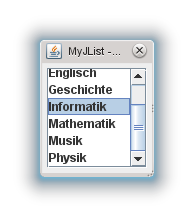
\includegraphics[width=1.0\textwidth]{./inf/SEKII/24_Java_GUI-Komponenten/JList_mit_ScrollPane.png}
\end{minipage}

\begin{lstlisting}
JScrollPane scrollPane = new JScrollPane();
scrollPane.setPreferredSize(new Dimension(WIDTH, HEIGHT));
contentPane.add(scrollPane);
JList<String> listFaecher = new JList<String>(faecherliste);
scrollPane.setViewportView(listFaecher);
\end{lstlisting}

\subsection{\myClass{JComboBox}}

Unter einer ComboBox versteht man eine Drop-Down-Auswahlliste. Im Unterschied
zu einer \myClass{JList}-Komponente nimmt die \myClass{JComboBox} vertikal immer
nur den Platz ein, der für die Darstellung des aktuell ausgewählten Elements
benötigt wird. Es gibt folglich auch keine Notwendigkeit für eine Einbettung in
eine \myClass{JScrollPane}. Auch kann man immer nur genau ein Element aus der
Liste auswählen.

\subsubsection{DefaultComboBoxModel}

Genau wie bei \myClass{JList} ist es für dynamische Inhalte nötig, ein
Daten-Modell zu benutzen:

\begin{lstlisting}
æString[] faecher = {"Englisch", "Deutsch", "Geschichte", 
                    "Mathematik", "Musik", "Physik"};
æDefaultComboBoxModel<String> faecherliste = new DefaultComboBoxModel<String>();
æJComboBox<String> comboboxFaecher = new JComboBox<String>(æfaecherlisteæ);
\end{lstlisting}

\begin{minipage}{0.5\textwidth}
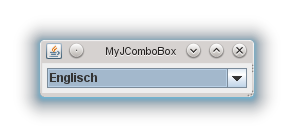
\includegraphics[width=0.8\textwidth]{./inf/SEKII/24_Java_GUI-Komponenten/JComboBox.png}
\end{minipage}
\begin{minipage}{0.5\textwidth}
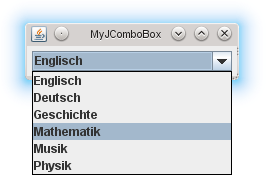
\includegraphics[width=0.8\textwidth]{./inf/SEKII/24_Java_GUI-Komponenten/JComboBox_ausgeklappt.png}
\end{minipage}

Die Methoden der Klasse \myClass{DefaultComboBoxModel} unterscheiden sich von
denen der Klasse \myClass{DefaultListModel}:

\bgroup
\def\arraystretch{1.2}
\begin{tabularx}{\textwidth}{|p{90mm}|X|}
\hline
\textbf{Methode} & \textbf{Erläuterung}
\\ \hline
\lstinline|  void addElement(Object element)| & 
Fügt das Element am Ende der Liste ein.
\\ \hline
\lstinline|* Object getElementAt(int index)| &
Liefert das Element an der angegebenen Position.
\\ \hline
\lstinline|  Object getSelectedItem()| &
Liefert das vom Benutzer ausgewählte Element.
\\ \hline
\lstinline|  int getSize()| &
Liefert die Größe der Liste zurück.
\\ \hline
\lstinline|* void insertElementAt(Object element, int index)| &
Fügt das Element an der angegebenen Position ein.
\\ \hline
\lstinline|  void removeAllElements()| & 
Löscht alle Elemente aus der Liste.
\\ \hline
\lstinline|* void removeElementAt(int index)| & 
Löscht das Element an der angegebenen Position.
\\ \hline
\lstinline|  void setSelectedItem(Object element)| & 
Ändert den Wert des aktuell vom Benutzer gewählten Elements. 
\\ \hline
\end{tabularx}
\egroup

\lstinline|(*) throws ArrayIndexOutOfBoundsException| 

Im Besonderen ist es so, dass bei der Verwendung von \myClass{JComboBox} auch
das Daten-Modell (\myClass{DefaultComboBoxModel}) eine Methode zur Verfügung
stellt, um das gewählte Element zu ermitteln, während es bei \myClass{JList} nur
über eine entsprechende Methode aus der Klasse \myClass{JList} (und nicht aus
der Klasse des Daten-Modells) geht. Man hat also die Wahl zwischen

\begin{lstlisting}
String gewaehltesFach = (String) comboboxFaecher.getSelectedItem();
\end{lstlisting}

und

\begin{lstlisting}
String gewaehltesFach = (String) faecherliste.getSelectedItem();
\end{lstlisting}
